\section{Data Stores and Consistency}
\label{sec:store-consistency}

The operational semantics of Fig.~\ref{fig:txnimp} allows operations
to witness arbitrary subsets of the global state, effectively mimicking the
behavior of an eventually consistent ({\sc ec}) data
store\footnote{Eventual consistency guarantees that in the absence of further
  updates, all reads witness the same global state
  \emph{eventually}. In any finite trace, however, there are no
  guarantees on what a read may witness.}. There are, however, data stores,
such as relational databases, that provide stronger consistency
guarantees than {\sc ec}. Like the isolation levels of transactions,
the consistency level of the underlying store also affects the
semantics of a program in non-trivial ways. In this section, we
demonstrate how the semantics of stronger stores with on-demand weak
isolation can be captured in our operational model. 

% A non-trivial $\I$ composed of isolation specifications from
% Fig.~\ref{fig:ansi-isolation} induces the machine to provide
% non-trivial isolation guarantees for transactions. However, weak
% isolation levels often only constrain the visibility sets of
% operations by dictating what \emph{not} to see; not what to see.  For
% instance, \iso{Repeatable Read} isolation prohibits operations of a
% transaction from witnessing different states. It, however, does not
% prohibit all operations of a transaction from witnessing an aribitrary
% subset of the global state. Consequently, the machine can remain an
% {\sc ec} store even while providing non-trivial isolation. How then to
% model the semantics of an {\sc sc} store, such as a relational
% database, with variable (weak) isolation?

First, we observe that the consistency level of a data store can be
captured by store-specific consistency constraints, along with
transaction-specific isolation constraints, via the trace invariant
$\I$. In particular, we can split $\I$ into two components: (1).
$\I_s$, the store-specific invariant, and (2). $\I_c$, the
program-specific (or, client-specific) invariant, to capture
consistency and isolation constraints, respectively.  $\I$ is now a
conjunction: $\I \,=\, \lambda\E.~\I_s(\E) \wedge \I_c(\E)$ (often
simplified to $\I \,=\, \I_s\wedge\I_c$).  While the program-specific
trace invariant ($\I_c$) is independent of the underlying data store,
the store specific invariant ($\I_s$) changes from store to store
depending on the consistency level.  For an eventually consistent
store, $\I_s$ is simply \emph{true}. Stronger stores, such as those
that support strong consistency, have non-trivial definitions for
$\I_s$.

A strongly-consistent {\sc sc} store guarantees a total order on all
operations w.r.t. $\visZ$ consistent with their chronological order. A
straightforward $\I_s$ for this store is the \C{SC} property
formalized below:
\begin{smathpar}
\begin{array}{l}
  \C{SC}(\E) \;=\; \forall\eta_1,\eta_2.~\{\eta_1,\eta_2\}
  \subseteq \E.\A \conj \id(\eta_1) < \id(\eta_2) \\
  \hspace*{2in}\Rightarrow \underE{\eta_1 \visar \eta_2}
\end{array}
\end{smathpar}
Unfortunately, $\I_s=\C{SC}$ conflicts with all isolation
specifications of Fig.~\ref{fig:ansi-isolation}. For instance,
consider a case where $\I_c(\E) \;=\; \forall
T_i.~\underE{\C{RC}(T_i)}$, a constraint that dictates all
transactions execute under \iso{Read Committed} isolation. Imagine a
sample execution where $\eta_1$'s transaction is not yet committed
when $\eta_2$ is generated. Letting $\eta_1$ be visible to $\eta_2$
violates $\I_c$, whereas not letting it be visible violates $\I_{s}$.
The only way to satisfy both invariants is to rule out all executions
that interleave the operations of one transaction with the other,
thereby enforcing serializability.  In general, when $\I_s$ conflicts
(but is not inconsistent) with $\I_c$, the only way to enforce both is
to restrict concurrency. Clearly, this is unacceptable since it
defeats the very purpose of supporting weak isolation. 
% How then do we enforce weak isolation on a strongly consistent
% machine?

In practice, relational databases resolve such conflicts by
prioritizing weak isolation (thus, concurrency and performance) over
strong consistency, so the execution traces do not necessarily satisfy
{\sc sc}. In particular, visibility constraints imposed by {\sc sc}
are violated iff they are found to be in conflict with the constraints
imposed by a transaction's isolation level. In the context of the
aforementioned example, $\eta_1$ is not made visible to $\eta_2$
because doing so would violate $\I_c$. However, if $\I_c$ is redefined
to \emph{true}, then the store makes $\eta_1$ visible to $\eta_2$ to
honor its consistency commitment\footnote{The term \emph{recency
commitment}~\cite{bailishat} is often used in practice to capture the
best-effort nature of {\sc sc}.}. We generalize this approach to any
$\I_s$ and $\I_c$ by defining a \emph{maximum visibility principle} to
determine an acceptable weakening of $\I_s$ in case of a conflict with
$\I_c$.  The principle requires the weakened consistency guarantee
($\I_s'$) of the store to enforce all visibility relationships imposed
by the actual consistency guarantee ($\I_s$), unless enforcing such a
relationship violates $\I_c$.
% The formal definition of the principle is relegated
% to the supplementary in the interest of space, but it can be
% understood in the context of an {\sc sc} store, where it weakens the
% store invariant to the following:
Formally:
\begin{definition}
$\I_s' : \E \rightarrow \Prop$ is said to be a maximum visibility
weakening of $\I_s : \E \rightarrow \Prop$ if and only if:
\begin{itemize}
  \item $\I_s'$ is weaker than $\I_s$: 
      $\forall\E.~ \I_s(\E) \Rightarrow \I_s'(\E)$, and
  \item In every trace $\E$ that satisfies $\I_c$, and for every pair
  of effects $\eta_1$ and $\eta_2$ in $\E$, if $\I_s(\E)$ requires
  $\eta_1$ to be visible to $\eta_2$, then so does $\I_s'(\E)$ unless
  extending $\E$ with $\visZ(\eta_1,\eta_2)$ violates
  $\I_c$:
  \begin{smathpar}
  \begin{array}{l}
  \forall\E,\eta_1,\eta_2.~ \I_c(\E) \Rightarrow (\I_s(\E)
    \Rightarrow \underE{\eta_1 \visar \eta_2}) \Rightarrow \\
    \hspace*{0.5in}(\I_s'(\E) \Rightarrow \underE{\eta_1 \visar
    \eta_2} \disj \neg\I_c(\E\,\cup\,(\emptyset,\{(\eta_1,\eta_2)\})))
  \end{array}
  \end{smathpar}
\end{itemize}
\end{definition}
Applying this principle, we can weaken {\sc sc} to obtain the
following store trace invariant ($\I_s$) for an {\sc sc} store whose
isolation constraints are captured by $\I_c$:
\begin{smathpar}
\begin{array}{lcl}
\I_s(\E) & = & \forall \eta_1,\eta_2.\, \{\eta_1,\eta_2\},
    \subseteq \E.\A \conj \id(\eta_1) <
    \id(\eta_2) \\
    & & \hspace*{0.5in} \Rightarrow 
      \underE{\eta_1 \visar \eta_2} \disj \neg\I_c(\E
    \cup (\emptyset,\{(\eta_1,\eta_2)\}))\\
\end{array}
\end{smathpar}
% GK : Please talk to me before changing the substance of the following paragraph.
$\I_s$ requires a trace $\E$ to satisfy the visibility constraints of
{\sc sc} except in cases where they are in conflict with $\I_c$.
Instantiating the parameter $\I$ with $\I_s \wedge \I_c$ in
Fig.~\ref{fig:txnimp} results in an operational semantics that
describes {\sc sc} stores with on-demand weak isolation, such as
provided by off-the-shelf relational databases. Similar approaches can be employed
to capture the semantics of other kinds of stores, such as a causally
consistent ({\sc cc}) data store, as specific instantiations of our
operational semantics\footnote{Details of the {\sc cc} instantiation
are given in the supplementary material.}.

%% \begin{remark}
%% Note that the purpose of maximum visibility principle is to
%% rationalize the observed behavior of databases in practice. In
%% particular, it is not intended to be a guiding principle to engineer
%% data stores.
%% \end{remark}

% \paragraph{A CC store} A causally consistent data store~\cite{gotsmanpopl16,LBC16}
% allows operations to only witness a causally consistent snapshot of the
% global state. The store-specific invariant obtained by weakening the
% {\sc cc} guarantee to account for conflicts with $\I_c$ is shown
% below (the original {\sc cc} does not contain the $\neg\I_c(\dots)$
% disjuncts): 
% \begin{smathpar}
% \begin{array}{lccl}
% \C{CC}(\E) & \;=\; &  & \forall \eta_1,\eta_2.\, 
%       \E \Vdash \eta_1 \soar \eta_2 \Rightarrow  \underE{\eta_1 \visar
%       \eta_2} \\
%     & & & \hspace*{0.6in}\disj \neg\I_c(\E \cup 
%                 (\emptyset,\{(\eta_1,\eta_2)\}))\\
%     &   & \wedge & \forall\eta_1,\eta_2,\eta_3.\,\underE{\eta_1 \visar
%       \eta_2} \conj \underE{\eta_2 \visoar \eta_3} \\
%     &   & &\hspace*{0.3in} \Rightarrow \underE{\eta_1 \visar \eta_3}
%       \disj \neg\I_c(\E \cup (\emptyset,\{(\eta_1,\eta_2)\}))\\
% \end{array}
% \end{smathpar}

% \noindent Instantiating the parameter $\I$  with $\I_s \wedge \I_c$ in
% Fig.~\ref{fig:txnimp} results in an operational semantics that admits
% violation of causal consistency if and only if the violation is
% inevitable to enforce $\I_c$.

    
\subsection{Weakly Consistent Replication}
\label{sec:replication}

\begin{figure}
\centering
\subcaptionbox {
  Replica model
  \label{fig:ec-theirs}
} [
  0.4\columnwidth
] {
  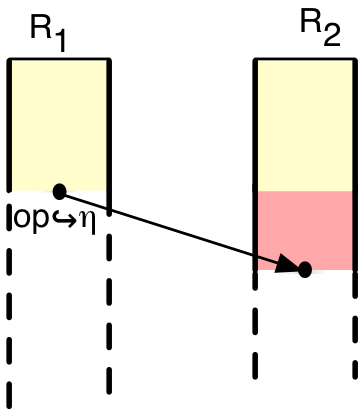
\includegraphics[scale=0.5]{Figures/ec-theirs}
 
}
\hspace*{0.1in}
\subcaptionbox {
  Subset model
  \label{fig:ec-ours}
}{
  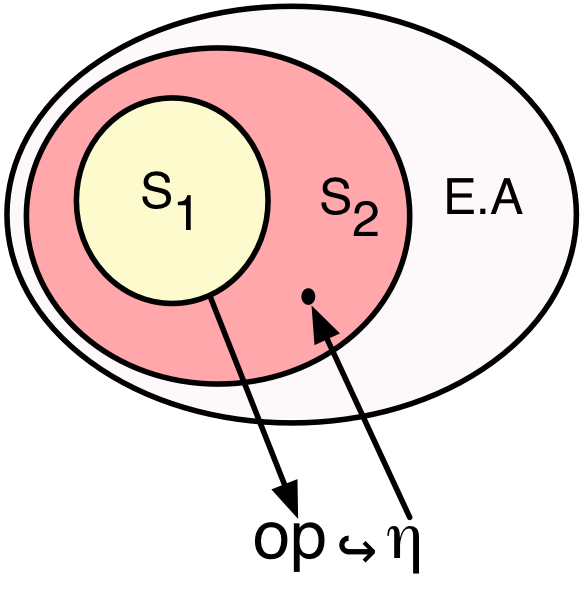
\includegraphics[scale=0.35]{Figures/ec-ours}
} \caption{\small In the replica model, operation $\op$ generates effect
$\eta$ at replica $R_1$, which is then merged to $R_2$. If the
\emph{store is {\sc cc}}, then $R_2$'s state at merge event is same or
larger than $R_1$'s state at generation event (the difference is
highlighted). In our subset model, $\op$ witnesses $S_1 \subseteq
\E.\A$ and generates $\eta$, which is immediately added to $\E.\A$. A
later operation may witness $S_2 \subseteq \E.\A$, and if the
\emph{operation is} {\sc cc} and $\eta \in S_2$, then it also
witnesses $S_1$ (i.e., $S_1 \subseteq S_2$). } 
% Moreover, Like $R_2 - R_1$, if all effects in $S_2 - S_1$ are
% concurrent with $\eta$, i.e., $\not\exists\eta'.~\eta' \in S_2 - S_1
% \conj % visZ(\eta,\eta')$, then any pre-condition $P$ that is valid
% when $\op$ executed is also valid when $\eta$ is witnessed because
% of the stability condition.
\label{fig:ec-theirs-vs-ours}
\end{figure}

Reasoning under weakly-consistent replication has received special
attention in recent work~\cite{gotsmanpopl16}. Our operational
semantics and proof system are general enough to admit replication as
a special case of our formulation. In this section, we explain how the
standard artifacts of weakly-consistent replication manifest in our
reasoning framework.

The primary challenge in this setting is to ensure that the
assumptions made and guarantees enforced by an operation at one
replica carry over to other replicas that merge their effects, thus
preserving the overall integrity of the system.  In prior
work~\cite{lbc16,gotsmanpopl16}, this challenge is partly addressed by
imposing restrictions on how various replica states differ, i.e., by
fixing a system model with a stronger baseline consistency ({\sc cc})
than {\sc ec}. This unfortunately restricts the reasoning approach
from being applied to data stores (e.g., \cite{bayou,pldi15}) that
provide guarantees weaker than causal consistency, such as causal
visibility or read-my-writes~\cite{zoo}. Causal consistency is not
baseline consistency in these stores because it is not \emph{highly
  available}~\cite{bailishat}.

Notably, our view of replication does not explicitly involve replicas.
Fig.~\ref{fig:ec-theirs-vs-ours} contrasts our model of
weakly-consistent replication with a conventional replica-based model.
Under our model, the notion of a replica is subsumed by the concept of
visibility; a replica is defined by the subset ($S$) of global state
($\E.\A$) that an operation witnesses. Constraints over replica states
therefore manifest as constraints over a specific visibility relation.
For example, instead of requiring the store to be causally consistent,
an operation can witness a causally consistent subset of the state;
such demands can be made via the trace invariant $\I$. For a
pre-condition ($P$) of the operation to be useful, it has to be an
assertion over every causally consistent subset of the global state.
Since any replica that eventually executes the operation has to expose
one such subset ($S$), the pre-condition is guaranteed to hold
regardless of the replica. There is however one problem with this
explanation - by considering subsets of just one global state, it
ignores the fact that the global state (hence, the replica states)
change during the execution of the operation. To account for such
changes, we might choose to distinguish between an effect generation
event at one replica $r_1$ and an effect merge event at replica $r_2$,
requiring that \emph{non-conflicting} operations execute between these
two events at $r_2$, and that they preserve certain
invariants~\cite{gotsmanpopl16}.  Instead, our framework folds all such
machinery into a stability condition predicated on $\I$
(\S\ref{sec:rely-guarantee}).  Since any change to the global state
during the execution of the operation is an interference, and $P$ is
required to be stable with respect to any such interference, it
follows that $P$ is valid on every replica, thus ensuring that
assumptions made at a generation event is also valid at the merge
event.

\subsection{Example}

We now consider the proof of the example in Fig.~\ref{fig:motiv-eg-1}
in greater detail. We assume an {\sc sc} store, such as a relational
database, whose store-specific trace invariant ($\I_s$) was shown
previously. Both transactions are run at {\sc si} isolation, hence
$\I_c$ is $\lambda\E.~\underE{\C{SI(Wd1)}} \conj
\underE{\C{SI(Wd1)}}$. As usual, $\I$ is $\I_s \conj \I_c$.

\begin{figure}
\centering
\begin{txnimpcode}
$\begin{decoration}
  \hspace*{0.3in}P : \{\neg\committed(\C{Wd1}) \conj \neg\committed(\C{Wd2}) \conj
                          \C{B} = \C{k}\}
\end{decoration}$

 $\begin{decoration}
 P_1:\{ \neg\committed(\C{Wd1}) \conj
        (\neg\committed(\C{Wd2}) \Rightarrow \C{B = k}) \conj\\
        \hspace*{0.3in}{\committed(\C{Wd2})} \Rightarrow 
            \C{Wd2} \wrstoar \C{B} \wedge \C{B = k-a2} \}
 \end{decoration}$
  txn$\langle$'Wd1'$\rangle${
              $\vdots$ 
     $\begin{decoration}
     \phi_4 : \{{\neg\committed(\C{Wd2})} \Rightarrow \C{B = k} \wedge \C{v3 = k-a1} \conj\\
        \hspace*{0.3in}({\committed(\C{Wd2})} \Rightarrow \C{Wd2}
        \wrstoar \C{B}) \conj \neg\committed(\C{Wd1}) \conj \\
        \hspace*{0.32in}{\committed(\C{Wd2})} \wedge
         {\C{Wd2} \visar \C{Wd1}} 
        \Rightarrow \C{B = k-a2} \wedge \\
        \hspace*{1.9in}\C{v3 = k-a2-a1}\}
     \end{decoration}$ 
     B := v3
     $\begin{decoration}
      \phi_5 : \{({\neg\committed(\C{Wd2})} \Rightarrow \C{B = k-a1}) 
          \conj \neg\committed(\C{Wd1}) \conj\\
         \hspace*{0.4in}{\committed(\C{Wd2})} 
            \Rightarrow \C{Wd2} \wrstoar \C{B} \wedge \C{B = k-a1-a2}\}
      \end{decoration}$ 
              $\vdots$ 
  }
 $\begin{decoration}
  Q_1 : \{{(\neg\committed(\C{Wd2})} \Rightarrow \C{B = k-a1})
            \conj \committed(\C{Wd1}) \conj\\
      \hspace*{0.4in}{\committed(\C{Wd2})} 
          \Rightarrow \C{B = k-a1-a2} \}
  \end{decoration}$ 

$\begin{decoration}
  \hspace*{0.3in}Q : \{\committed(\C{Wd1}) \conj \committed(\C{Wd2}) \conj
                          \C{B} = \C{k-a1-a2}\}
\end{decoration}$
\end{txnimpcode}
\vspace*{-8pt}
\caption{\small \C{Wd1} transaction decorated with assertions}
\label{fig:wd1-decorated}
\vspace*{-12pt}
\end{figure}

Decorated parts of \C{Wd1} relevant to the discussion are shown in
Fig.~\ref{fig:wd1-decorated}.  \C{Wd2} is similar and not
shown\footnote{The supplementary material shows the fully decorated program.}.
Temporary name \C{v3} has been introduced to capture the result of the
RHS expression \C{C-a1}.  Assertions implicitly refer to the current
execution ($\E$), just as Hoare triples implicitly refer to the
current state.  The context for propositions is also the implicit,
i.e., we write $\psi$ instead of $\underE{\psi}$. The proposition \C{k
$\ge$ a1+a2} remains an invariant, hence elided. The pre-condition
$P_1$ of \C{Wd1} accounts for the possibility of \C{Wd2} committing
before \C{Wd1}, writing \C{k-a2} to \C{B}. Since neither \C{Wd1} nor
\C{Wd2} are committed at the beginning, the pre-condition $P$ of the
program is extended with $\neg\committed(\C{Wd1}) \wedge
\neg\committed(\C{Wd2})$, from which $P_1$ follows. The post-condition
$Q_1$ of \C{Wd1} asserts different values for \C{B} depending on
whether or not \C{Wd2} has already committed.  It also asserts that
\C{Wd1} has committed. The post-condition $Q_2$ of \C{Wd2} (not shown)
is similar, but with the roles of \C{Wd1} and \C{Wd2} exchanged. The
post-condition $Q$ follows from $Q_1 \wedge Q_2$, hence valid. It
remains to show that \C{Wd1} satisfies its specification (\C{Wd2} must
also satisfy its spec, but the proof is similar).

First, we focus on the sequential aspect of the proof and show that
the assertions that decorate \C{Wd1} are indeed valid. We consider the
triple associated with the assignment to \C{B} for illustration. The
pre-condition $\phi_4$ asserts different values for \C{B} and \C{v3}
(temporary alias of RHS expression) depending on whether or not
\C{Wd2} is committed. Inside \C{Wd1}, $\committed(\C{Wd2})$ may mean
that either \C{Wd2} happened before \C{Wd1} (hence can be visible to
all of \C{Wd1}), or that it committed concurrently with \C{Wd1} (hence
cannot be visible to all of \C{Wd2}).  Nonetheless, $\phi_4$ only
considers the case when $\C{Wd2} \visar \C{Wd1}$. As we show below,
this is sufficient to prove the post-condition $\phi_5$, which appears
to make a stronger claim about the value of \C{B}. The proof follows
from the RG rule \rulelabel{RG-Asgn} for assignments, which allows us
to easily conclude the following about the execution state after the
assignment:\vspace*{-12pt}

\begin{smathpar}
\begin{array}{l}
    {\neg\committed(\C{Wd1}) \conj \C{Wd1} \wrstoar \C{B} 
    \conj (\neg\committed(\C{Wd2})} \Rightarrow \C{B = k-a1}) \conj\\
    ({\committed(\C{Wd2})} \Rightarrow \C{Wd2} \wrstoar
    \C{B}) \conj \\
    ({\committed(\C{Wd2})} \wedge {\C{Wd2} \visar \C{Wd1}} 
    \Rightarrow \C{B = k-a2} \wedge \C{B = k-a2-a1})
\end{array}
\end{smathpar}

\noindent The rule also lets us assume that the execution satisfies trace
invariant ($\I$), which asserts {\sc si} for both transactions.  Since
both transactions now write to \C{B}, {\sc si} requires either
$\C{Wd1} \visar \C{Wd2}$, or $\C{Wd2} \visar \C{Wd1}$. Since \C{Wd1}
is not yet committed ($\neg\committed(\C{Wd1})$), {\sc si} (which
subsumes {\sc rc}) prohibits the former possibility, allowing us the
deduce $\C{Wd2} \visar \C{Wd1}$. This lets us derive
${\committed(\C{Wd2})}  \Rightarrow \C{B = k-a2} \wedge \C{B =
k-a2-a1}$, allowing us to prove the post-condition $\phi_5$.

The second part of the proof is to show that assertions are stable
despite the interference from the the concurrent thread executing
\C{Wd2}. We formalize the interference as a rely relation that
describes the semantics of \C{Wd2} at just the right level of
abstraction. In particular, we would like to capture two important
facts about \C{Wd2}: 
\begin{itemize}
  \item  If \C{Wd2} commits, then it should have already written to
  \C{B}. This fact is needed to show that \C{Wd2} conflicts with
  \C{Wd1}, so that \C{SI(Wd1)} property can be exploited to deduce
  $\C{Wd2} \visar \C{Wd1}$ from $\committed(\C{Wd2})$ in the
  sequential proof.

  \item The value written to \C{B} is either $\C{k-a1-a2}$ or
  $\C{k-a1}$ depending on whether or not \C{Wd1} has already
  committed. This is clearly necessary to deduce the value of \C{B}
  before and after \C{Wd1} commits.
\end{itemize}
 The resultant rely relation ($R_1$) is shown below (note: we
write $(\E'-\E) \Vdash {\committed(\C{Wd2})}$ to express that \C{Wd2}
is not committed in $\E$, but committed in $\E'$.):

\begin{smathpar}
\begin{array}{lcl}
  R_1 & = & \{ (\E,\E') \;|\; \neg\underE{\committed(\C{Wd1})} \conj
        (\E'-\E) \Vdash {\committed(\C{Wd2})}\\
%       \neg\underE{\committed(\C{Wd2})} \conj \I(\E) \conj \I(\E')\\
%       \conj (\E'-\E) \subseteq \C{Wd2} \conj \\
%   & & \hspace*{0.5in} \E' \Vdash \committed(\C{Wd2}) ~\Rightarrow~ \E'
%       \Vdash \C{Wd2} \wrstoar \C{B} \conj \\ 
%   & & \hspace*{0.5in} \underE{\committed(\C{Wd1})} \conj \E' \Vdash
%   \committed(\C{Wd2}) \Rightarrow \C{B=k-a1-a2} \\
%   & & \hspace*{0.5in} \neg\underE{\committed(\C{Wd1})} \conj
%       (\E'-\E) \Vdash {\committed(\C{Wd2})}\\
    & & \hspace*{0.8in}\Rightarrow \C{B=k-a2} \conj 
        \E' \Vdash \C{Wd2} \wrstoar \C{B} \\
    & & \hspace*{0.37in} \conj \underE{\committed(\C{Wd1})} \conj
        (\E'-\E) \Vdash {\committed(\C{Wd2})}\\
%       \C{COMMIT(Wd2)} \in (\E'.\A-\E.\A) \\
    & & \hspace*{0.6in}\Rightarrow \C{B=k-a1-a2} \conj
        \E' \Vdash \C{Wd2} \wrstoar \C{B} \\
    & & \hspace*{0.37in}\conj \forall(\eta \in \E'.\A - 
        \E.\A).~\txn(\eta) = \C{Wd2}\}\\
\end{array}
\end{smathpar}
For the sake of completeness, we also explicitly represent the fact
that all the effects added by $R_1$ are of \C{Wd2}. This is needed to
prove that an interference from \C{Wd2} does not affect the local
state of \C{Wd1}.

The stability for $\phi_4$ w.r.t. $R_1$ is trivial to establish: if
$R_1$ does not commit \C{Wd2}, then the value of \C{B} is unaffected,
and if it commits \C{Wd2}, then $\C{Wd2}\not\visar\C{Wd1}$, hence
$\phi_4$ doesn't care. For $\phi_5$, {\sc si} condition should be used
to show that any interference from \C{Wd2} is invalid. The proof
proceeds on the same lines as the Hoare proof discussed above; it is
also discussed in detail in \S\ref{sec:motivation}.

The final aspect of the proof is to show that any interference from
\C{Wd1} is contained in its guarantee relation $G_1$, which is also
the rely relation $R_2$ for \C{Wd2}. Since the implementation of
\C{Wd2} is same as \C{Wd1}, $R_2$ (hence $G_1$) is same as $R_1$ shown
above, but with \C{Wd2} and \C{Wd1} interchanged. Continuing our focus
on the assignment statement, the guarantee proof requires us to show
that if executing the assignment takes the execution from $\E$ to
$\E'$, such that $\E'$ satisfies $\I$, then $(\E,\E') \in G_1$.  The
proof follows from the \rulelabel{RG-Asgn} rule, which establishes
that (a). the assignment statement does not commit \C{Wd2}, and (b).
it adds a write effect $\eta$ such that $\txn(\eta)=\C{Wd1}$. This
finishes the proof for the triple in focus. The proofs for other
triples of \C{Wd1} can also be constructed similarly. The combination
of correctness proofs for \C{Wd1} and \C{Wd2} yields a correctness
proof for the program.

% \paragraph{Discussion.} As evident from the example, instantiating the
% proof system for a specfic combination of consistency and isolation
% settings, and then deriving facts specific to that setting
% characterizes our reasoning approach. While intuition suggests that
% some instantiations, such as {\sc sc} with ANSI SQL isolation, are
% general enough to cover many practical cases, it not the case in
% reality given the subtle differences in the semantics of isolation
% levels among different database implementations. For instance,
% Postgres' \iso{Repeatable Read} isolation is stronger than ANSI SQL's
% or MySQL's in non-trivial ways.  Furthermore, the need for high
% availability on geo-replicated stores has led to the development of
% new isolation levels which are yet to be standardized. For example,
% \emph{Parallel Snapshot Isolation}~\cite{psi} was proposed in 2011,
% and \emph{Non-Monotonic Snapshot Isolation}~\cite{nmsi} in 2013, both
% targeted for replicated stores. As more commercial weakly consistent
% stores adopt variants of transactions, like the recently introduced
% \emph{lightweight transactions} of Cassandra, it is reasonable to
% expect new isolation definitions to continue to be proposed.  While it
% is possible to carefully engineer a reasoning framework for each
% combination of consistency and isolation, such a strategy would lead
% to multiple semantic definitions and proof systems with no obvious way
% to compare and relate them.  Having a parameterized semantics and a
% proof framework built on the such semantics allows us to support these
% variants as distinct, yet comparable instantiations, thus avoiding the
% need for semantics re-engineering every time an
% application is retargeted to a new platform.

%   A distinguishing feature of our framework is that it
%   is parameteric over different isolation and consistency
%   instantiations, whose properties can be encapsulated within the
%   trace invariant $\I$.  While it is true that most relational
%   databases implement standard ANSI SQL isolation levels similar to
%   the ones shown in Fig.~\ref{fig:ansi-isolation}, there is no clear
%   agreement on the exact semantics of these isolation levels on
%   various weakly-consistent stores.  Thus, what Oracle calls
%   serializable isolation is a slightly stronger variant of snapshot
%   isolation.  Having a parameterized semantics and proof framework
%   built on this semantics allows us to support these variants
%   without the need for semantics re-engineering every time an
%   application is retargeted to a new platform.

%   Moreover, the need for high availability on geo-replicated stores
%   is incentivizing the development of new isolation
%   levels. \emph{Parallel Snapshot Isolation}, for example, was
%   proposed in 2011, and \emph{Non-Monotonic Snapshot
%     Isolation}~\cite{...} in 2013, both for replicated
%   stores. Commercial eventually-consistent stores have only just
%   started adopting transactions (the first release of Cassandra with
%   support for multi-key transactions is slated for later this year),
%   and all indications are that we should expect to see new isolation
%   instantiations in the future.  Without parameterization, we would
%   need to carefully engineer a reasoning framework for each
%   isolation and consistency variant.  Clearly, each such framework
%   would be incomparable to one another. On the other hand, our
%   treatment allows us to accommodate the myriad of different
%   isolation and store-consistency instances without the need for
%   bespoke specialization.



